% Created 2025-01-14 Tue 17:49
% Intended LaTeX compiler: pdflatex
\documentclass[letterpaper, 14pt]{article}
\usepackage[utf8]{inputenc}
\usepackage[T1]{fontenc}
\usepackage{graphicx}
\usepackage{longtable}
\usepackage{wrapfig}
\usepackage{rotating}
\usepackage[normalem]{ulem}
\usepackage{amsmath}
\usepackage{amssymb}
\usepackage{capt-of}
\usepackage{hyperref}
\usepackage{minted}
\usepackage{xcolor}
\usepackage{hyperref}
\usepackage{tocloft}
\usepackage{minted}
\usemintedstyle{manni}
\usepackage{pdfpages}
\usepackage{fancyhdr}
\usepackage{graphicx}
\usepackage[top=1.4in, left=0.5in, right=0.5in, bottom=0.8in]{geometry}
\usepackage[T1]{fontenc}
\usepackage{helvet}
\pagestyle{fancy}
\renewcommand{\headrulewidth}{0pt}
\renewcommand{\footrulewidth}{0pt}
\setlength{\parindent}{0em}
\setlength{\parskip}{1em}
\usepackage{hyperref}
\usepackage {color}
\usepackage {tabularray}
\usepackage{xcolor}
\hypersetup{
colorlinks=true,
linkcolor=blue,
filecolor=magenta,
urlcolor=cyan,
citecolor=green,
pdfborder={0 0 0}
}
\usepackage[most]{tcolorbox}
\author{Hilduara Abreu}
\date{\today}
\title{School Year 2024-25 | Principal Message January 2025}
\hypersetup{
 pdfauthor={Hilduara Abreu},
 pdftitle={School Year 2024-25 | Principal Message January 2025},
 pdfkeywords={},
 pdfsubject={},
 pdfcreator={Emacs 29.4 (Org mode 9.6.15)}, 
 pdflang={English}}
\begin{document}

\fancyfoot[C]{\setlength{\unitlength}{1in}\begin{picture}(5,0)\put(-1.8,-0.5){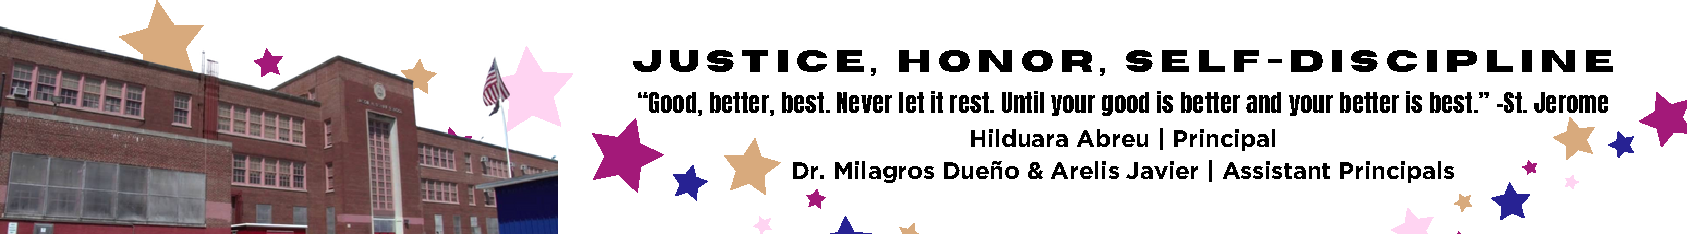
\includegraphics[width=8.8in,height=1.3in]{logo-1}}\end{picture}}
\fancyhead[C]{\setlength{\unitlength}{1in}\begin{picture}(5,0)\put(-1.9,-0.5){
\includegraphics[width=8.9in,height=1.3in]{logo-2}}\end{picture}}
\fancyhead[R]{\thepage}
\pagenumbering{gobble}

\begin{document}
\newpage
\vspace*{-0.2cm}
\emph{\textbf{Subject: Welcome to January, 2025 at PS 192: The School of Joyful Learning!}}

Dear PS192 Families,

Happy New Year!

I extend my warmest wishes for a healthy, peaceful, and successful start to 2025. At P.S. 192, we firmly believe that learning is a collaborative effort between home and school. I sincerely thank you for your continued dedication and involvement in your child’s education.

The start of a new year presents an excellent opportunity to embrace new habits and set meaningful goals that can enhance both your life and your child’s academic journey. It is also a time to reflect on areas where growth and improvement are possible.

We have an exciting month ahead, filled with opportunities for learning and engagement. I encourage you to participate in the upcoming events:

Parent Association Meeting
\begin{itemize}
\item Date: January 14
\item Time: 8:00 a.m.
\item Location: Library
\end{itemize}

School Leadership Team (SLT) Meeting
\begin{itemize}
\item Date: January 22
\item Time: 2:30 p.m. to 5:30 p.m.
\end{itemize}

Coffee with the Principal
\begin{itemize}
\item Date: January 31
\item Time: 8:00 a.m.
\item Location: Library
\end{itemize}

I look forward to seeing you at this month’s events and continuing our partnership to support student success.

With Justice, Honor, and Self-Discipline,


\includegraphics[width=0.2\textwidth]{hil_signature}

\textbf{Hilduara Abreu, Principal}

\textbf{The School of Joyful Learning!}

\href{www.ps192.org}{www.ps192.org}

\newpage

\fancyfoot[C]{\setlength{\unitlength}{1in}\begin{picture}(5,0)\put(-1.8,-0.5){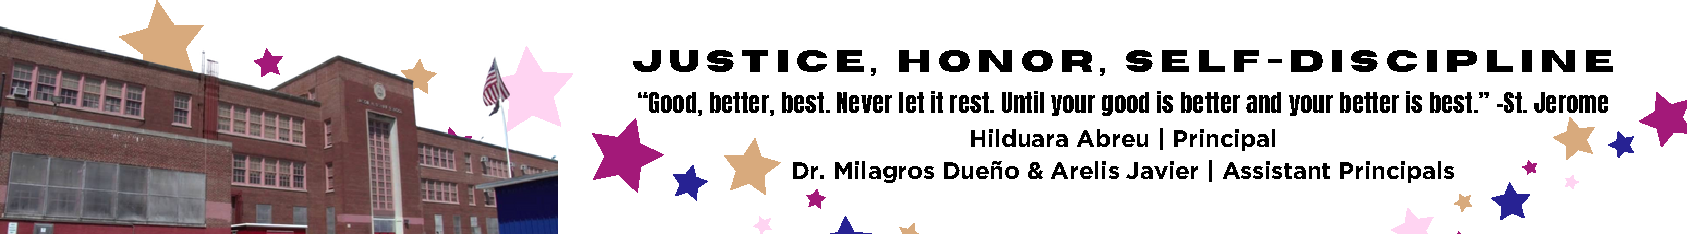
\includegraphics[width=8.8in,height=1.3in]{logo-1}}\end{picture}}
\fancyhead[C]{\setlength{\unitlength}{1in}\begin{picture}(5,0)\put(-1.9,-0.5){
\includegraphics[width=8.9in,height=1.3in]{logo-2}}\end{picture}}
\fancyhead[R]{\thepage}
\pagenumbering{gobble}

\begin{document}
\newpage
\vspace*{-0.2cm}

\emph{\textbf{Asunto: Bienvenidos a enero de 2025 en PS 192: ¡La Escuela del Aprendizaje Alegre!}}

\textbf{Estimados padres y tutores},

¡Feliz Año Nuevo!

Les extiendo mis más cálidos deseos para un comienzo saludable, pacífico y exitoso en el 2025. En la P.S. 192, creemos firmemente que el aprendizaje es un esfuerzo colaborativo entre el hogar y la escuela. Les agradezco sinceramente por su continuo compromiso e involucramiento en la educación de su hijo/a.

El inicio de un nuevo año presenta una excelente oportunidad para adoptar nuevos hábitos y establecer metas significativas que puedan mejorar tanto su vida como el trayecto académico de su hijo/a. También es un momento para reflexionar sobre las áreas donde se puede crecer y mejorar.

Tenemos un mes emocionante por delante, lleno de oportunidades para aprender y participar. Les animo a participar en los próximos eventos:

Reunión de la Asociación de Padres
\begin{itemize}
\item Fecha: 14 de enero
\item Hora: 8:00 a.m.
\item Ubicación: Biblioteca
\end{itemize}

Reunión del Equipo de Liderazgo Escolar (SLT)
\begin{itemize}
\item Fecha: 22 de enero
\item Hora: 2:30 p.m. a 5:30 p.m.
\end{itemize}

Café con la Directora
\begin{itemize}
\item Fecha: 31 de enero
\item Hora: 8:00 a.m.
\item Ubicación: Biblioteca
\end{itemize}

Espero verlos en los eventos de este mes y continuar nuestra colaboración para apoyar el éxito de los estudiantes.

Con justicia, honor y autodisciplina,


\includegraphics[width=0.2\textwidth]{hil_signature}

\textbf{Hilduara Abreu, Principal}

La escuela del aprendizaje allegro!

\href{www.ps192.org}{www.ps192.org}
\end{document}
